\documentclass{amsart}

\usepackage[a4paper,margin=2cm]{geometry}
\usepackage{tikz}
\usetikzlibrary{automata}
\usepackage{float}
\tikzset{every node/.style={align=center}, >= latex, font=\scriptsize}

\title{Why is the Bouncing Ball Hybrid Automaton not a Rectangular Hybrid Automaton?}
\begin{document}
\maketitle
The hybrid system representing a bouncing ball can be represented as the following hybrid automaton:
\begin{figure}[H]
    \begin{center}
        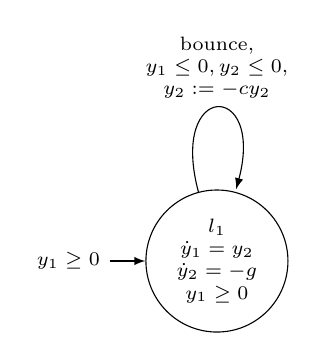
\begin{tikzpicture}[node distance=4cm,initial text={$y_{1}\geq 0$}]
            \node [state,initial] (s0) {$l_{1}$ \\ $\dot{y}_{1}=y_{2}$\\$\dot{y}_{2}=-g$ \\ $y_{1}\geq0$};
            \path[->] (s0) edge [loop above] node [above] {bounce, \\$y_{1}\leq0,y_{2}\leq0$,\\ $y_{2}:=-cy_{2}$} (s0);
        \end{tikzpicture}
    \end{center}
\end{figure}
In detail we have that
\begin{align*}
    V & =\{y_{1},y_{2}\} \\
    L & =\{\ell_{1}\} \\
    A & =\{\text{bounce}\} \\
    Init & =\{(\ell_{1},y_{1}\geq0)\} \\
    Inv(\ell_{1}) & =\{y_{1}\geq 0\} \\
    E & =\{e_{1}=(\ell_{1},\text{bounce },\ell_{1})\}  \\
    r(e_{1}) & = \{y_{2}:=-cy_{2}\} \\
    g(e_{1}) & = \{y_{1}\leq0,y_{2}\leq0\} \\
    f(\ell_{1}) & =\{\dot{y}_{1}=y_{2},\dot{y}_{2}=-g\}
\end{align*}
The continuous variable $y_{1}$ denotes the vertical position of the ball and $y_{2}$ denotes the vertical velocity. $g$ is the gravitational acceleration and $c\in[0,1]$ is the constant indicating the loss of energy with each bounce. So after the bounce the speed of the ball will be $c$ times the speed of the ball before the bounce, and in the opposite direction.

The reason why the bouncing ball hybrid automaton cannot be abstracted to a rectangular hybrid automaton is that the flow of $y_{1}$ is not a rectangular set but a function evaluating $y_{2}$ dependent on time.
\end{document}
